\chapter{Background}
\label{cha:background}

In this chapter, we provide an overview of the main concepts, paradigms and technologies that are relevant for the purpose of this work.
We start by introducing the concept of \textbf{Public Cloud Providers} and the \textbf{Multi Cloud paradigm}.
We then provide a brief overview of \textbf{Kubernetes}, the de-facto standard for container orchestration. 
After that, \textbf{Krateo PlatformOps}, an open-source Kubernetes-based platform that is a fundamental part of our system, is introduced.
We deemed also valuable to provide an overview of the existing works in the field of \textbf{multi-cloud resource management}. 
Finally, the \textbf{GreenOps landscape} is introduced, focusing on the the \textbf{Computational Sustainability} initiatives by Public Cloud Providers and on \textbf{carbon-aware systems for resource management}. 

\section{Public cloud providers}

The Cloud Computing definition by the National Institute of Standards and Technology (NIST) \cite{nist} states that ``\textit{Cloud Computing is a model for enabling ubiquitous, convenient, on-demand network access to a shared pool of configurable computing resources (e.g., networks, servers, storage, applications, and services) that can be rapidly provisioned and released with minimal management effort or service provider interaction}" \cite{nist}.
\textbf{Public Cloud Providers} or Cloud Service Providers (CSPs) are companies that have as their core business the provisioning of cloud computing services. These services, which are growing in number and complexity, range from computing resources to storage, networking, databases, machine learning, and more. 


%Public cloud is a deployment model opposed to private cloud.
%The former deployment model allows organizations to consume cloud services without having to build and maintain their own physical infrastructure, therefore reducing capital expenditure (CapEx) and shifting to an operational expense model (OpEx). 

%The public cloud represents a multi-tenant environment where resources are shared among multiple customers.
%Doing so requires public cloud provider to leverage paradigm and technique which were known in the industry well before the advent of cloud computing: virtualization and isolation.



Currently, as of 2024, the public cloud market is dominated by three main hyperscalers: \textbf{Amazon Web Services (AWS)}, \textbf{Microsoft Azure}, and \textbf{Google Cloud Platform (GCP)}.
An hyperscaler is ...

Figure \ref{fig:pcp} shows the worldwide market share of leading cloud infrastructure service providers as of Q3 2024 \cite{statista}.

\begin{figure}[htb]
    \centering
    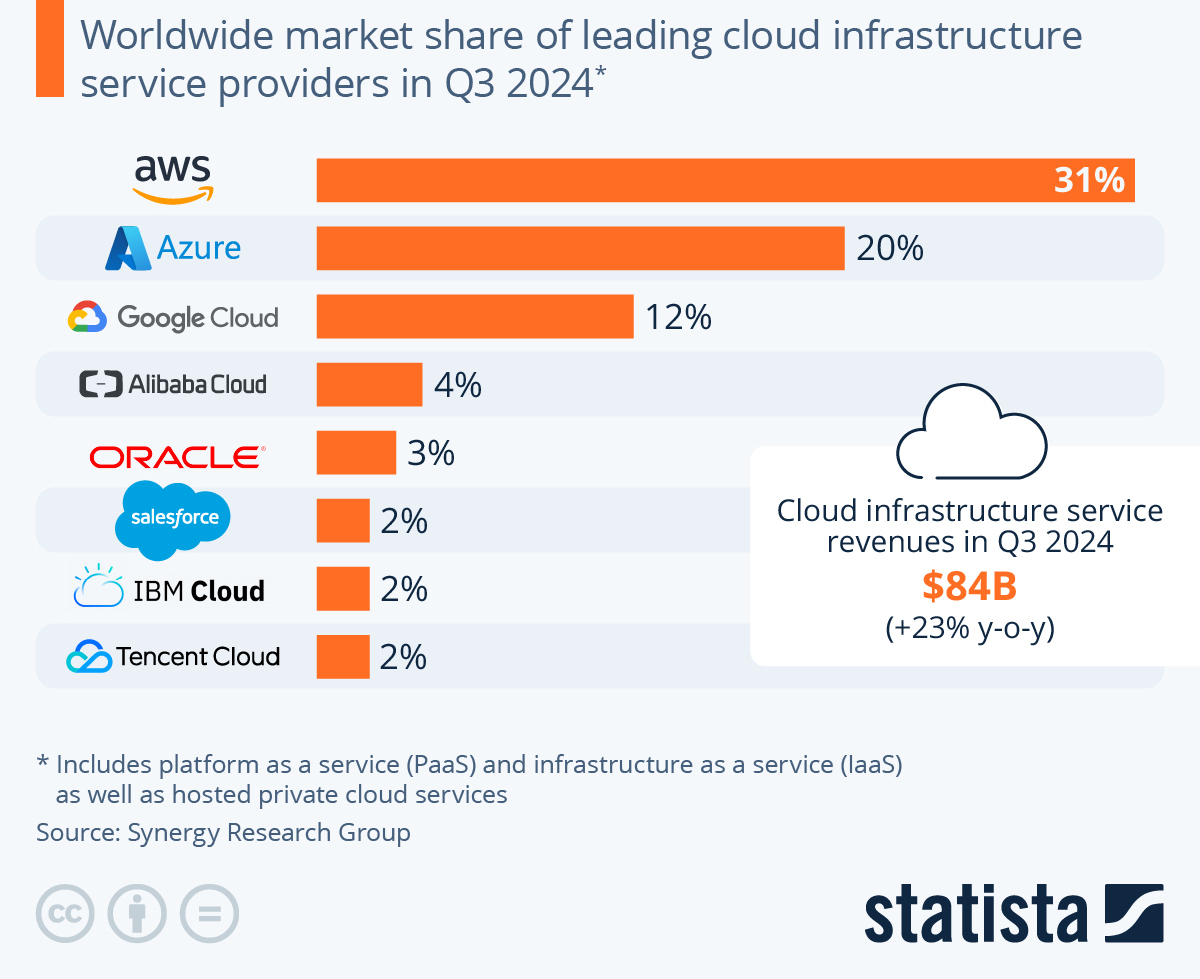
\includegraphics[width=0.75\linewidth]{images/pcp.jpeg}
    \caption{Worldwide market share of leading cloud infrastructure service providers as of Q3 2024 \cite{statista}}
    \label{fig:pcp}
\end{figure}
  


% https://www.statista.com/chart/18819/worldwide-market-share-of-leading-cloud-infrastructure-service-providers/


\subsection{Regions and zones}
cloud regions
regions vs availability zones
Cloud providers usually further divide region into ...
Each Region supports a subset of the available instance types.
We could safely assume that our workload specs are quite standard and therefore can be scheduled on any cloud region.

each provider has a different number of regions and zones and different naming conventions
there is no standardization in the industry for this. 
for instance a region located in london is called eu-west-2 in AWS, uk-west in Azure and europe-west2 in GCP

[table how many regions per cloud provider]

Figure \ref{fig:azure_data_centers} shows the geo-distribution of Azure cloud regions (data centers) and the country Grid Carbon Intensity (year 2024) as reported by Electricity Maps \cite{electricity_maps}. Data center coordinates were retrieved by an Azure CLI command dump \cite{azure_data_centers_information}.

\begin{figure}[htb]
    \centering
    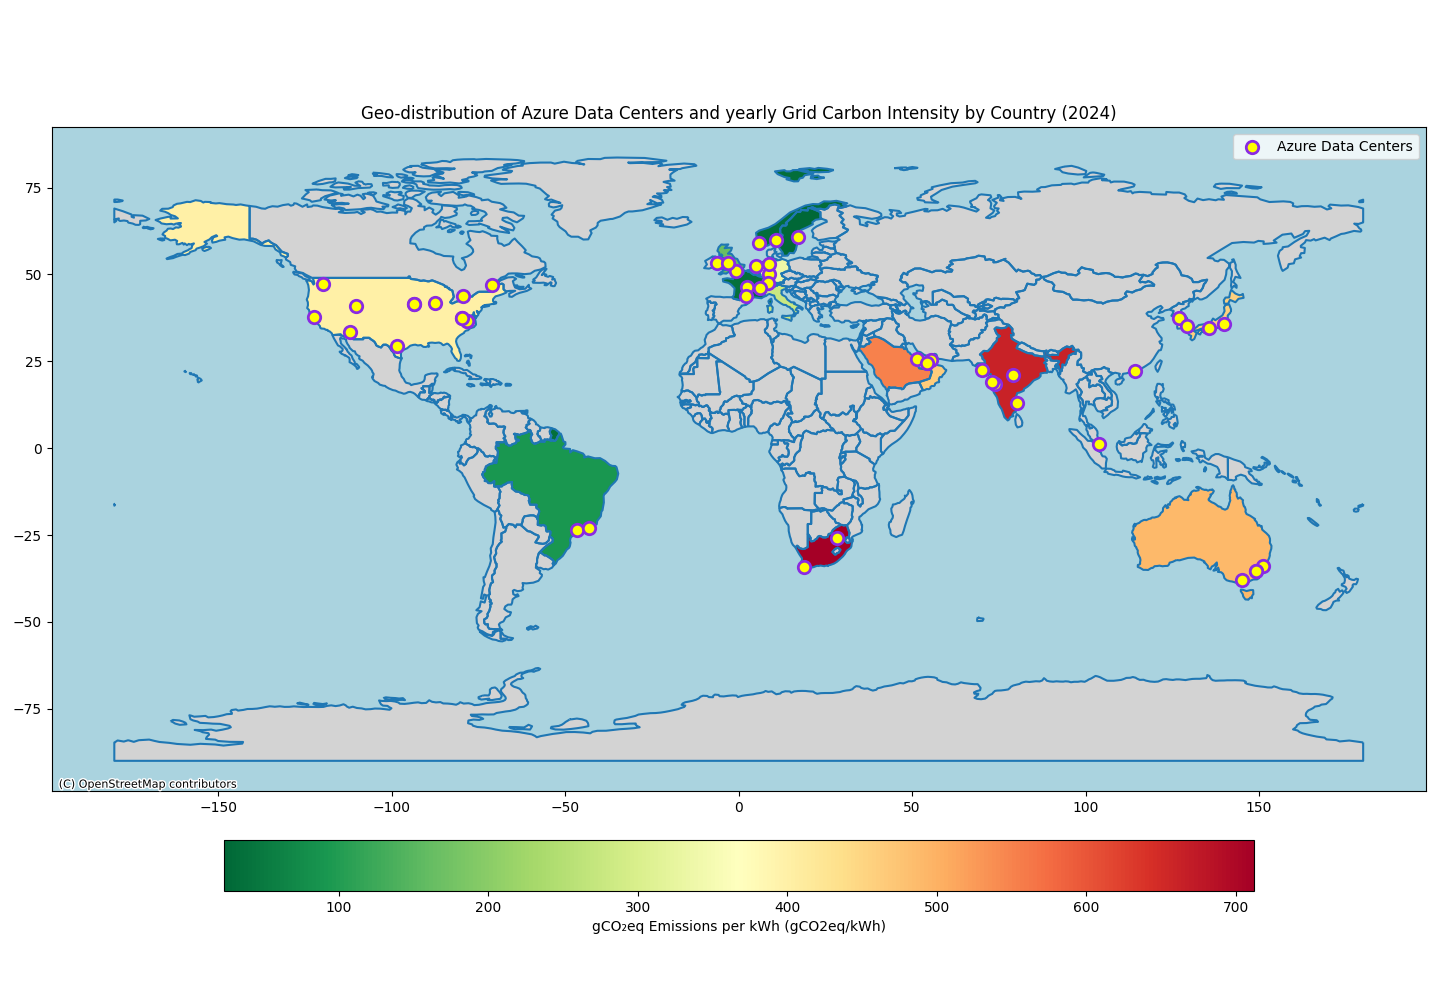
\includegraphics[width=1\linewidth]{images/azure_data_centers.png}
    \caption{Geo-distribution of Azure data centers with country Grid Carbon Intensity}
    \label{fig:azure_data_centers}
\end{figure}

% https://www.naturalearthdata.com/downloads/110m-cultural-vectors/


\subsection{Multi cloud paradigm}

what is multi cloud paradigm

why is useful
how to achieve

advantages of multi-cloud
flexibility
risk reduction (reduces vendor lock-in)

why it is important for the organizations


disadvantages
increased complexity
attack surface increased (security)




Why multi-cloud in the context of our system?
Different cloud providers have data centers in various locations around the world. This diversity allows for more options when geographically shifting workloads to regions with lower carbon intensity.
However the 3 big players have a big overlap: each one is present almost everywhere.
Multi-cloud paradigm could be leveraged for lowering costs.
For basic use cases, we can even set a single cloud provider to be used (e.g., Azure) and therefore just a multi-region environment.
Being able to work in a multi-cloud environment is also important for accomplishing user / company needs: they can use just a single cloud provider or more than one for different reasons. Therefore if our system supports more cloud providers, it will accomplish more users' needs.
If the system is designed to be multi-cloud then flexibility is higher for organizations and users.
For the purpose of this work, we will consider only the 3 major Public Cloud Provider as of today: AWS, Azure, GCP

\section{Kubernetes}

Kubernetes is an open-source platform for automating the orchestration of containerized applications.
It is widely used in the industry and became the de-facto standard for container orchestration.
An extensive description of Kubernetes is out of the scope of this thesis but it is deemed necessary to provide a brief overview of the main concepts of Kubernetes that are relevant for the purpose of this work.
Figure \ref{fig:kubernetes_architecture} shows the Kubernetes architecture as described by the Cloud Native Computing Foundation (CNCF) \cite{kubernetes_cnfc}.

\begin{figure}[htb]
    \centering
    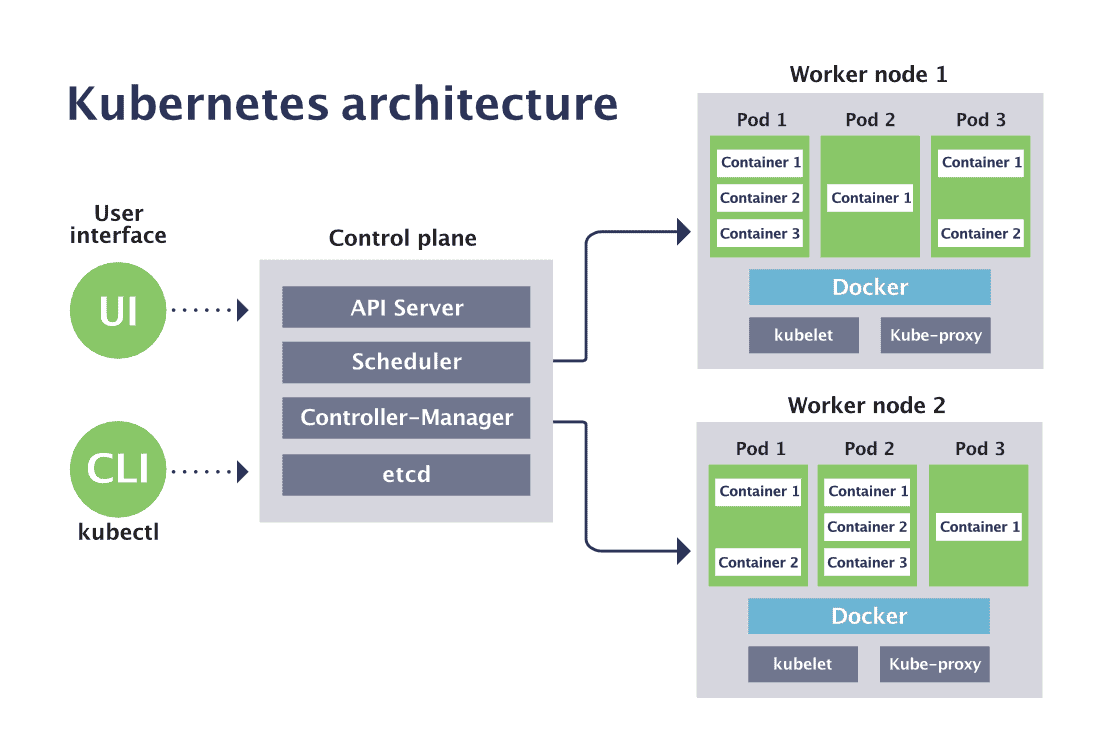
\includegraphics[width=1\linewidth]{images/kubernetes-architecture-diagram.png}
    \caption{Kubernetes architecture by CNCF \cite{kubernetes_cnfc}}
    \label{fig:kubernetes_architecture}
\end{figure}

The main components of Kubernetes are:
\begin{itemize}[itemsep=0.2pt, topsep=1pt]
    \item[$\bullet$] \textbf{Kubernetes API server}: the central component that manages the Kubernetes cluster. It exposes the Kubernetes API and is responsible for validating and mutating data for the Kubernetes objects.
    \item[$\bullet$] \textbf{etcd}: a key-value store used to store the cluster state.
    \item[$\bullet$] \textbf{Kubernetes controller manager}: a daemon that embeds the core control loops shipped with Kubernetes.
    \item[$\bullet$] \textbf{Kubernetes scheduler}: a component that assigns Pods to nodes.
    \item[$\bullet$] \textbf{Kubelet}: an agent that runs on each node in the cluster. It makes sure that containers are correctly running in a Pod.
    \item[$\bullet$] \textbf{Kubernetes proxy}: a network proxy that runs on each node in the cluster. It maintains network rules and it is responsible for routing network traffic.
    \item[$\bullet$] \textbf{Container runtime}: the software that is responsible for running containers on the Node (in this case represented by Docker).
\end{itemize}

[TO BE FIXED]
It must be noted that in our system we are not extending the Kubernetes scheduler as described for instance in the work of ..
since we are not dealing with the scheduling of the in-cluster resources (e.g., Kubernetes Pods). 
We are instead focusing on the management of external resources on cloud providers.
As described in the following section, our focus will be on the Kubernetes API sever and in particular on Admission Control 

\subsection{Kubernetes as a platform}

[TO BE FIXED]
Kubernetes as a platform to manage external resources
representing resources as kubernetes objects to leverage the powerful kubernetes API and tooling

This concept is widely used 
(cloud provider operators for example)
% https://aws.amazon.com/it/blogs/containers/kubernetes-as-a-platform-vs-kubernetes-as-an-api-2/

Many cloud-native development teams work with a mix of configuration systems, APIs, and tools to manage their infrastructure. This mix is often difficult to understand, leading to reduced velocity and expensive mistakes. Config Connector provides a method to configure many Google Cloud services and resources using Kubernetes tooling and APIs.
%(https://cloud.google.com/config-connector/docs/overview)

%https://cloud.google.com/config-connector/docs/concepts/resources#managing_resources_with_kubernetes_objects

\subsection{Kubernetes extendability}

[TO BE FIXED]
% https://www.cncf.io/blog/2022/06/15/kubernetes-operators-what-are-they-some-examples/

Kubernetes allows for the extension of its functionalities through the use of \textbf{Custom Resource Definitions (CRDs)} and \textbf{Kubernetes Operators}, effectively adopting the so-called \textbf{Operator paradigm}.
Simply put, Custom Resource Definitions are a way to instruct Kubernetes to manage a new resource type. They are a schema that defines the structure of the resource and the Kubernetes API server will validate the resource against the schema.
\textbf{Custom Resources (CRs)} are actually instances of the resources defined by CRDs and are managed by an Operator.
The Operator is a piece of software that is responsible for managing the lifecycle of the resources defined by the CRD.
Effectively the code of an Operator is usually deployed on the Kubernetes cluster in the form of a Deployment.
This concept is not different of what actually happens for standard built-in Kubernetes resources which are however manged by built-in controllers.
An high-level overview of the Operator paradigm is depicted in Figure \ref{fig:operator_paradigm}.

\begin{figure}[H]
    \centering
    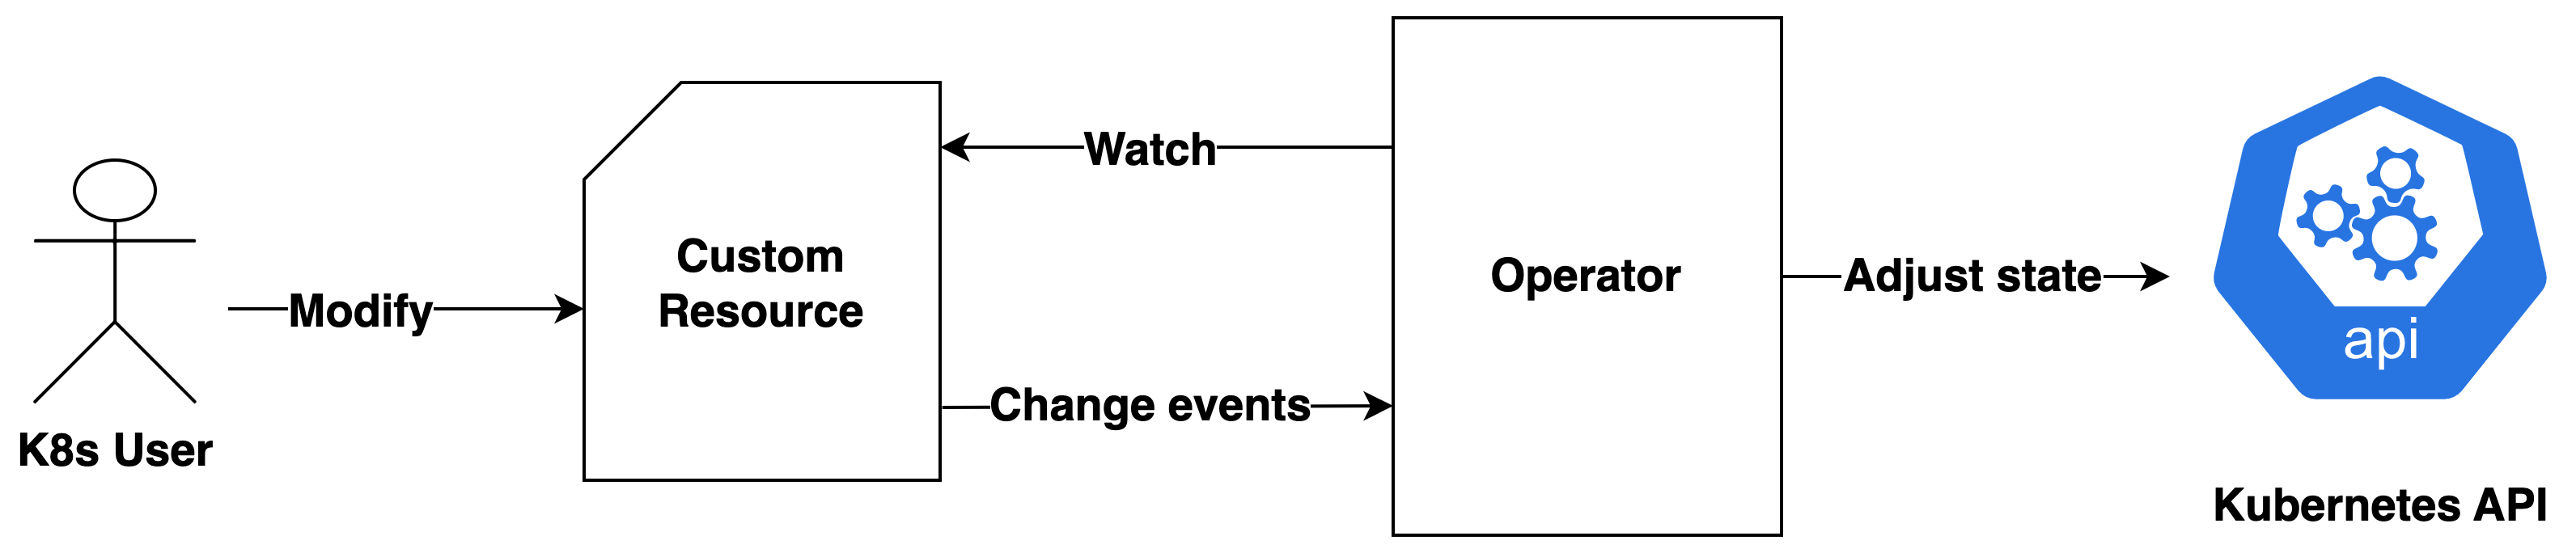
\includegraphics[width=1\linewidth]{images/opeartor_paradigm.png}
    \caption{Operator paradigm}
    \label{fig:operator_paradigm}
\end{figure}

\subsection{Helm}

Helm is a \textbf{package manager} for Kubernetes. Therefore with Helm it is possible to define, install and manage Kubernetes applications in a simpler way compared to a manual management of Kubernetes resources manifests \cite{helm}.
Helm is a graduated project in the CNCF and it is the de-facto standard for Kubernetes package management.
The key concept is the \textbf{Helm chart}, which is a collection of files that describe a related set of Kubernetes resources. 
These files are mainly of two types: templates and values.
The \textbf{templates} are Kubernetes manifest files that are rendered by Helm's \textbf{powerful templating engine}. 
The \textbf{values} are the set of variables that are used to render the templates.
Upon an Helm chart installation, Helm will render the templates ``injecting" the values and deploy the resources in the Kubernetes cluster. 
One major advantage that Helm provides is the complete management of the lifecycle of the resources.
As a matter of fact, Helm allows to easily \textbf{upgrade}, \textbf{rollback} and \textbf{uninstall} the Kubernetes resources deployed with a Helm chart reducing time and errors in such operations \cite{helm}. 
Without Helm, the user would have to deal with each single Kubernetes resource manifest file and manually apply changes to them.
Finally, users can benefit of Helm charts already developed by the community and leverage chart distribution within their organization using Helm repositories.

\section{Krateo PlatformOps}
\label{sec:krateo}

Krateo PlatformOps (Krateo) is an \textbf{open-source Kubernetes-based platform} that aims to provide a unified interface for managing any desired resource on any infrastructure \cite{krateo_docs}.
Krateo runs as a Kubernetes deployment inside a Kubernetes cluster but \textbf{acts as a control plane} even for resource external to the Kubernetes cluster.
The only requirement for this management is that the resources need to be logically descriptible using a YAML file which represents the desired state of the resources \cite{krateo_docs}.
% Platform engineering
% Developer platform: a unified environment providing tools, services, and infrastructure that enables teams to efficiently build, test, and deploy software without managing underlying complexity. This complexity is handled by the platform team.
% Recognized by Gartner. Gartner said ... by 2025 companies without a ... (cite)
Krateo is composed of three main parts:
\begin{itemize}[itemsep=0.2pt, topsep=1pt]
    \item[$\bullet$] Krateo Composable Operations
    \item[$\bullet$] Krateo Composable Portal
    \item[$\bullet$] Krateo Composable FinOps
\end{itemize}

For the purpose of this work, we will focus on the \textbf{Krateo Composable Operations} part, which is the core of the Krateo platform and is responsible for managing the lifecycle of resources in a Kubernetes cluster \cite{krateo_docs}.
Krateo Composable Operations is composed in turn by several components. Due to their core importance in our system, as described in section XYZ we will briefly describe the functionalities of the \textbf{Krateo core-provider} and the \textbf{Krateo composition-dynamic-controller}.

\subsection{Krateo core-provider}

The Krateo core-provider is a Kubernetes operator that has the duty of downloading and managing Helm charts. It first checks for the existence of a file named \textit{values.schema.json} in the chart folder and uses it to generate a Kubernetes Custom Resource Definition (CRD), accurately representing the possible values that can be expressed for the installation of the chart \cite{krateo_core_provider}.
The file \textit{values.schema.json} is a JSON schema that describes the structure of the \textit{values.yaml} file for the related Helm chart and it is considered a standard best practice for Helm charts. It basically provides a way to validate the \textit{values}.yaml file before the Helm chart is installed (i.e., to check if the values are in the correct format).
In other words, the Krateo core-provider operator is responsible for deploying the Helm chart as a \textbf{native Kubernetes resource}, which allows for the management of the Helm chart lifecycle through Kubernetes APIs \cite{krateo_docs}.
As a matter of fact, out of the box, Kubernetes does not provide a way to manage Helm charts natively and the Krateo core-provider is one tool that allows to do so.
The Kubernetes Custom Resource Definition introduced by the Krateo core-provider is called \textbf{\textit{CompositionDefinition}}. It is a CRD that represents the Helm chart and its values (a Helm Chart archive (.tgz) with a JSON Schema for the values.yaml file) \cite{krateo_core_provider}.
Upon a CompositionDefinition manifest application to the Kubernetes cluster, the Krateo core-provider generates the CRD from the schema defined in the \textit{values.schema.json} file included in the chart. It then deploys an instance of the Krateo composition-dynamic-controller, setting it up to manage resources of the type defined by the CRD \cite{krateo_core_provider}.

\subsection{Krateo composition-dynamic-controller}

The Krateo composition-dynamic-controller is the Kubernetes operator that is instantiated by the Krateo core-provider to manage the Custom Resources whose Custom Resource Definition is generated by the core-provider.
In practice, when a Custom Resource (CR) is created, the instance of composition-dynamic-controller checks if a Helm release associated with the CR already exists in the cluster \cite{krateo_composition_dynamic_controller}. 
If this is not the case, it performs an \textit{helm install} operation using the values specified in the CR to create a new Helm release. This will practically deploy all the resources defined in the Helm chart using \textbf{Helm's templating engine}.
However, if the Helm release does already exist, it instead executes an \textit{helm upgrade} operation, updating the release's values with those specified in the CR, effectively updating the resources in the cluster.
Finally, when the CR is deleted from the cluster, the instance of the composition-dynamic-controller performs an \textit{helm uninstall} on the release, removing all the resources defined in the Helm chart from the cluster \cite{krateo_composition_dynamic_controller}. \\

The architecture of the Krateo core-provider and composition-dynamic-controller is depicted in Figure \ref{fig:krateo_core_provider}.

\begin{figure}[htb]
    \centering
    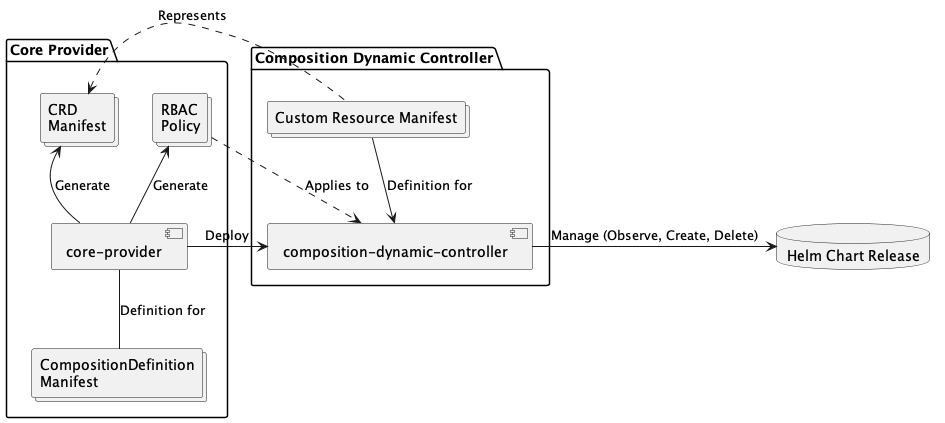
\includegraphics[width=1\linewidth]{images/kraeto_core_provider.png}
    \caption{Krateo core-provider and composition-dynamic-controller architecture \cite{krateo_core_provider}}
    \label{fig:krateo_core_provider}
\end{figure}

\section{Multi cloud resource management}
\label{sec:multi_cloud_resource_management}

The idea of a \textbf{dynamic management of workloads leveraging a multi-cloud paradigm} is not new. In this section we will provide an overview of some of the existing works in the literature that have tackled the problem of multi-cloud resource management.

\subsection{Dynamic Virtual Machine placement}
The work of Simarro et al. \cite{Simarro_2011} back at the dawn of cloud computing (2011) proposed a multi-cloud architecture for the dynamic placement of Virtual Machines (VMs).
The main objective of the system was cost optimization but this paradigm provides reliability and flexibility as well.
The scheduling part is comprised of a ``\textbf{cloud broker}" that is responsible for VM placement \textbf{transparent to users} providing a single uniform interface to the cloud resources.
Users can provide to the system a ``\textbf{service description template}'' to specify the number of VMs to provision and some constraints.
The cloud broker architecture is composed of two major components: the \textbf{scheduler} and the \textbf{cloud manager} \cite{Simarro_2011}. The former is responsible for placement decision across multiple cloud providers, while the latter is responsible for the actual management of the VMs in the cloud providers. More precisely, the cloud manager is represented by the OpenNebula (ONE) virtual infrastructure manager \cite{Simarro_2011}.
OpenNebula is an open-source platform that aims to provide a unified management interface for multiple virtualization technologies and cloud providers \cite{open_nebula}.

\subsection{Cloud service brokers}
A CSB is a system that acts as an \textbf{intermediary} between cloud service providers and consumers, providing a \textbf{unified interface} to manage cloud resources across multiple providers \cite{Wadhwa_2013}.
Cloud service brokers (CSBs) were described and categorized by Wadhwa et al. \cite{Wadhwa_2013} in their work of 2013.
The emerging market of cloud computing led to the proliferation of cloud services and providers, and by consequence the need for mechanisms to manage costs, capacity and resources \cite{Wadhwa_2013}. 

An interesting CSB example in the literature is the \textbf{STRATOS} system by Pawluk et al. proposed in 2012. The work can be considered a pioneer in the field of multi-cloud resource management since it can be framed in the first years of cloud computing \cite{STRATOS} but the proposed paradigms and concepts are relevant today.
STRATOS tried to \textbf{avoid the assumption of resource homogeneity} and represented an initial attempt to provide a ``\textbf{cross-cloud resource provisioning}'' system \cite{STRATOS}.
The proposed architecture enables the specification of high-level objectives that can be assessed in a standardized manner across different providers. The decision-making process is fully automated, shifting the decision point from deployment to runtime \cite{STRATOS}.
Users first submit a topology document, triggering the Cloud Manager to communicate with the Broker for topology instantiation. The Broker (implemented in Java) then conducts the initial resource acquisition decision (RAD), optimizing the allocation of resources across multiple providers (configured beforehand) \cite{STRATOS}.
Experiments indicate that distributing workloads across different cloud providers can reduce the overall cost of the topology. The approach taken by the authors primarily focuses on two objectives: \textbf{cost efficiency} and \textbf{avoiding vendor lock-in}. The application environment was deployed on public cloud platforms, specifically AWS and Rackspace \cite{STRATOS}.

\subsection{AI-based resource management in cloud computing}
\label{sec:ai_based_resource_management}

More recent works have focused on the development of systems that leverage AI techniques for the optimization of resource management in cloud computing environments.

[Machine learning (ML)-centric resource management in cloud computing: A review and future directions]
% https://www.sciencedirect.com/science/article/abs/pii/S1084804522000649

[HUNTER: AI based holistic resource management for sustainable cloud computing]
% https://www.sciencedirect.com/science/article/abs/pii/S0164121221002211

\subsection{Policy-driven resource management systems}

[SLA-driven dynamic cloud resource management]
% https://www.sciencedirect.com/science/article/abs/pii/S0167739X1300215X

[Deadline-aware Dynamic Resource Management in Serverless Computing Environments]
% https://ieeexplore.ieee.org/abstract/document/9499407

[Policy-Based Cloud Management Through Resource Usage Prediction]
% https://link.springer.com/chapter/10.1007/978-3-319-13464-2_14

[Amazon Web Services Cloud Compliance Automation with Open Policy Agent]
% https://ieeexplore.ieee.org/abstract/document/10612535


---

% Optimizing Cost and Maximizing Profit for Multi-Cloud-Based Big Data Computing by Deadline-Aware Optimize Resource Allocation
% https://link.springer.com/chapter/10.1007/978-981-15-8469-5_3

\section{GreenOps landscape}

what is greenops

greenops landscape 

In the context of cloud-native sustainability,
the Technical Advisory Group (TAG) Environmental Sustainability is a XYZ that supports and advocates for environmental sustainability initiatives in cloud native technologies.

% https://hbr.org/2020/09/how-green-is-your-software

% https://www.usenix.org/publications/loginonline/slos-and-ghgs

\subsection{Green Software foundation}

green software foundation
very important actor in the field of green software

sci: https://sci.greensoftware.foundation/

proposed a standard for data like the FOCUS standard available 
trying to push a specification similar to what focus is for FinOps
as per 2025 this standard is not yet adopted by cloud providers
``real time cloud" proposed standard (not yet adopted): https://github.com/Green-Software-Foundation/real-time-cloud?tab=readme-ov-file

the foundation also developed the Impact Framework which will be described in section XY
could be potentially integrated in our system

https://patterns.greensoftware.foundation/catalog/cloud/choose-region-closest-to-users
[which patterns are used in our system]

\subsection{Computational Sustainability by Public cloud providers}

what are they already doing

---

We assume that a cloud data center will likely rely on the same energy sources that characterize a specific geographical region (grid).
For example, if data from Electricity Maps tell us that Finland is producing energy with low carbon emissions then we assume that the data centers in that area will likely be powered with energy from low carbon sources.
However, some cloud providers may have better access to renewable energy sources in certain regions due to their individual initiatives e.g. wind farms that feed directly into their data centers.


what microsoft is already doing with alternative energy sources apart from grid


---

https://blog.google/inside-google/infrastructure/data-centers-work-harder-sun-shines-wind-blows/

Google CFE\%: “This is the average percentage of carbon free energy consumed in a particular location on an hourly basis, while taking into account the investments we have made in carbon-free energy in that location. This means that in addition to the carbon free energy that's already supplied by the grid, we have added carbon-free energy generation in that location”.



\section{Carbon-aware systems for resource management}

Having provided an overview of the existing works in the field of multi-cloud resource management and having introduced the GreenOps landscape, we now focus on the state of the art in the field of carbon-aware systems for resource management.

The work of 2023 by Sukprasert et al. named ``\textit{Spatiotemporal Carbon-aware Scheduling in the Cloud: Limits and Benefits}'' \cite{10.1145/3599733.3606301} is a comprehensive analysis on the limits and benefits of the employment of geographical shifting and time shifting for cloud workloads.
The authors highlight the fact that different workloads have different characteristics and therefore different degrees of flexibility. Those include, for instance: \textbf{execution deadlines}, \textbf{data protection laws}, and \textbf{latency requirements}. Therefore, carbon savings are constrained by a complex set of factors that need to be taken into account when designing a carbon-aware system \cite{10.1145/3599733.3606301}.

\subsection{CASPER}

CASPER (Carbon-Aware Scheduling and Provisioning for Distributed Web Services) is a carbon-aware scheduling and provisioning system whose primary purpose is to minimize the carbon footprint of distributed web services \cite{Souza_2023}.
The system is defined as a multi-objective optimization problem that considers two factors: the \textbf{variable carbon intensity} and the \textbf{latency constraints} of the network \cite{Souza_2023}.
By evaluating the framework in real-world scenarios, the authors demonstrate that CASPER achieves significant reductions in carbon emissions (up to 70\%) while meeting application \textbf{Service Level Objectives (SLOs)}, highlighting its potential for practical implementation in large-scale distributed systems \cite{Souza_2023}.
The authors of CASPER highlight the importance of considering the workload characteristics such as memory state, \textbf{latency} and \textbf{regulatory constraints such as GDPR} \cite{Souza_2023}.
The system is not adopting time-shifting since it is dealing with web services that are by their nature non-stopping workloads. The architecture is tied to scheduling K8s resources inside K8s clusters and does not consider external resource management.
%https://github.com/carbonfirst/casper?tab=readme-ov-file
%[HOW is it deployed]

\subsection{CASPIAN}

[TO BE ADDED]

\subsection{Let'sWaitAwhile}

[TO BE ADDED]

\subsection{CarbonScaler}

[TO BE ADDED]

https://dl.acm.org/doi/abs/10.1145/3626788
CarbonScaler: Leveraging Cloud Workload Elasticity for Optimizing Carbon-Efficiency

\subsection{Microsoft's Carbon-Aware Kubernetes}

[TO BE ADDED]
[https://devblogs.microsoft.com/sustainable-software/carbon-aware-kubernetes/]


\subsection{A Low Carbon Kubernetes Scheduler}
[TO BE ADDED]
https://ceur-ws.org/Vol-2382/ICT4S2019_paper_28.pdf

It provisions entire K8s clusters on the selected regions.
Interesting feature: they use local air temperature and solar irradiance as tiebreaker for 2 datacenters with similar carbon intense grid. The claim is that: “Solar irradiance varies more widely than carbon intensity across global regions” and that “Local air temperature surrounding a datacentre affects the amount of energy needed for cooling”. 


---

Data-driven Algorithm Selection for Carbon-Aware Scheduling
https://hotcarbon.org/assets/2024/pdf/hotcarbon24-final23.pdf


Carbon aware computing at Google
https://www.performance2021.deib.polimi.it/www.performance2021.deib.polimi.it/wp-content/uploads/2021/11/Carbon-Aware-Computing-%40-Google-and-Beyond.pdf
Year: 2021
Description: 
It states that Carbon-aware computing is: exploiting flexibility in when and where and how computing is done to reduce carbon emissions.
Some examples of flexible workloads are: video processing, training large-scale machine learning models, simulation pipelines.
The components they recognized to be necessary are: accurate carbon intensity data (Tomorrow), Scalable infrastructures (Cloud), Virtualizations and migration mechanisms (VMs), Well identified flexible load, data-driven methodology.
At Google: the total amount of work that needs to get done per day is quite predictable.



\subsection{State of the Art analysis outcome}

many simulation compared to real-world scenarios
no much flexibility for what concern variaty of resource managed
usually tied to one type of resource (e.g., VMs, K8s pods)

usually either time shifting or geographical shifting

\newpage
